\documentclass[dvipdfmx, a4paper, 11pt]{jsarticle}

% --- 日本語環境用設定 ---
\usepackage[top=25truemm,bottom=25truemm,left=25truemm,right=25truemm]{geometry}

% --- 追加パッケージ ---
\usepackage[dvipdfmx]{graphicx} % 画像読み込み用
\usepackage{booktabs}           % 表の罫線を美しくする
\usepackage{url}                % URLの表示
\usepackage{float}              % 図表の位置固定 [H] 用
\usepackage{amsmath}            % 数式

\graphicspath{{../results/}}

% --- 箇条書き設定（パッケージを使わない方法に変更）---
\renewcommand{\labelitemi}{--}

% --- タイトル情報 ---
\title{分析1 小レポート：\\メディア利用と政治的信頼の実証分析\\ \large{―ISSP・WVSデータによるOLS対Random Forest比較（確定版）―}}
\author{明治大学 政治経済学部 杉本ゼミ\\ 牧野 杏珠}
\date{\today}

\begin{document}

\maketitle

\begin{abstract}
本レポートは，卒業論文第4部・分析1（既存アンケート調査データによる実証分析）の
結果を要約する内部メモである。ISSP「Role of Government」日本サブセット
（$N=4{,}091$，1996/2006/2016年）とWVS Time Series日本サブセット
（$N=9{,}523$，1981--2019年）に対し，単純なOLS線形回帰に加え，Random Forest
・SHAP・$K$-meansクラスタリングを用いた分析を行った。結論は一貫している：
モデルを非線形的に高度化し，雇用状態や主観的所得水準といった「経済的破壊の
当事者性」を捉える変数を追加してもなお，年齢・学歴・政治的関心等の利用可能な
変数群では政治的信頼・効力感の分散のごく一部しか説明できない。個人単位の
SNS利用頻度（WVS Wave 7）を直接投入した場合も，議会・公務員信頼のいずれに
対しても統計的に有意な効果は確認されなかった（日・米・独で頑健，英国のみ例外）。
本レポートは卒論本文（\texttt{sections/04\_empirical.tex}）の該当箇所と
整合するよう作成されており，数値はすべて\texttt{results/}以下の実行結果
ファイルから直接転記している。
\end{abstract}

\section{分析の目的と位置づけ}
分析1は，「メディア利用（特にSNS利用）が政治的信頼に与える影響」という
マクロな量的関係を，既存の大規模社会調査の個票データを用いて検証するもの
である。本稿全体の核心的課題である「Ricci (2020) のルサンチマン理論は
日本に適用できるか」という問いに対し，分析1はその前半——経済的破壊の
当事者性やSNS利用が，制度への信頼という態度指標にどう表れるか——を担当する。

\section{データと方法}

\subsection{データセット}
\begin{itemize}
  \item ISSP「Role of Government」（ZA4747）日本サブセット：$N=4{,}091$，
    1996年・2006年・2016年の3時点。
  \item WVS Time Series（Wave 1--7統合，バージョン3.0）日本サブセット：
    $N=9{,}523$，1981--2019年。メディア利用頻度はWave 6（2010年）・
    Wave 7（2019年）のみ調査。SNS利用（\texttt{E253B}）はWave 7のみ。
\end{itemize}

\subsection{分析手法}
OLS線形回帰に加え，非線形性・交互作用を捉えるためRandom Forest回帰
（5分割交差検証によるR\textsuperscript{2}比較）とSHAP値による特徴量寄与度の可視化を
行った。さらに，回答者の政治的態度プロファイル（政治的有効性感覚の欠如・
公務員信頼・汚職認識・政治的関心）に基づく$K$-meansクラスタリング
（$K=2$--$6$でシルエット係数を比較し$K=3$を採用）を実施した。説明変数には，
年齢・性別・学歴・政治的関心・調査年に加え，Ricciの経済的破壊の当事者性を
捉える代理変数として，ISSPでは雇用状態（\texttt{WORKYN}：完全失業／
非労働力人口），WVSでは雇用状態と主観的所得水準（\texttt{X047R\_WVS}，
低・中・高の3段階）を追加した。

\section{結果：ISSP分析}

\subsection{OLSとRandom Forestの予測性能比較}
表\ref{tab:ml-comparison}の通り，政治的有効性感覚の欠如・公務員信頼・
汚職認識のいずれについても，Random ForestはOLSをわずかに上回るのみで，
いずれのモデルもR\textsuperscript{2}が0.06を超えることはなかった。

\begin{table}[H]
\centering
\caption{ISSP：OLS対Random Forestの5分割交差検証R\textsuperscript{2}比較}
\label{tab:ml-comparison}
\begin{tabular}{lccc}
\toprule
目的変数 & OLS R\textsuperscript{2} & RF R\textsuperscript{2} & 差分(RF$-$OLS) \\
\midrule
政治的有効性感覚の欠如 (no\_say, $N=3650$) & 0.0566 & 0.0574 & $+0.0007$ \\
公務員への信頼 (trust\_civil, $N=3543$) & 0.0321 & 0.0397 & $+0.0076$ \\
汚職認識 (corruption, $N=2431$) & 0.0208 & 0.0305 & $+0.0097$ \\
\bottomrule
\end{tabular}
\end{table}

SHAP分析（図\ref{fig:shap-civil}）では，公務員信頼への寄与が最も大きいのは
年齢と政治的関心であり，追加した雇用状態のうち「非労働力人口」は学歴・
性別より大きい寄与を示した一方，「完全失業」の寄与はほぼゼロだった
（$N=4{,}091$中わずか78名，1.9\%と少数のため検出力を欠く）。

\begin{figure}[H]
    \centering
    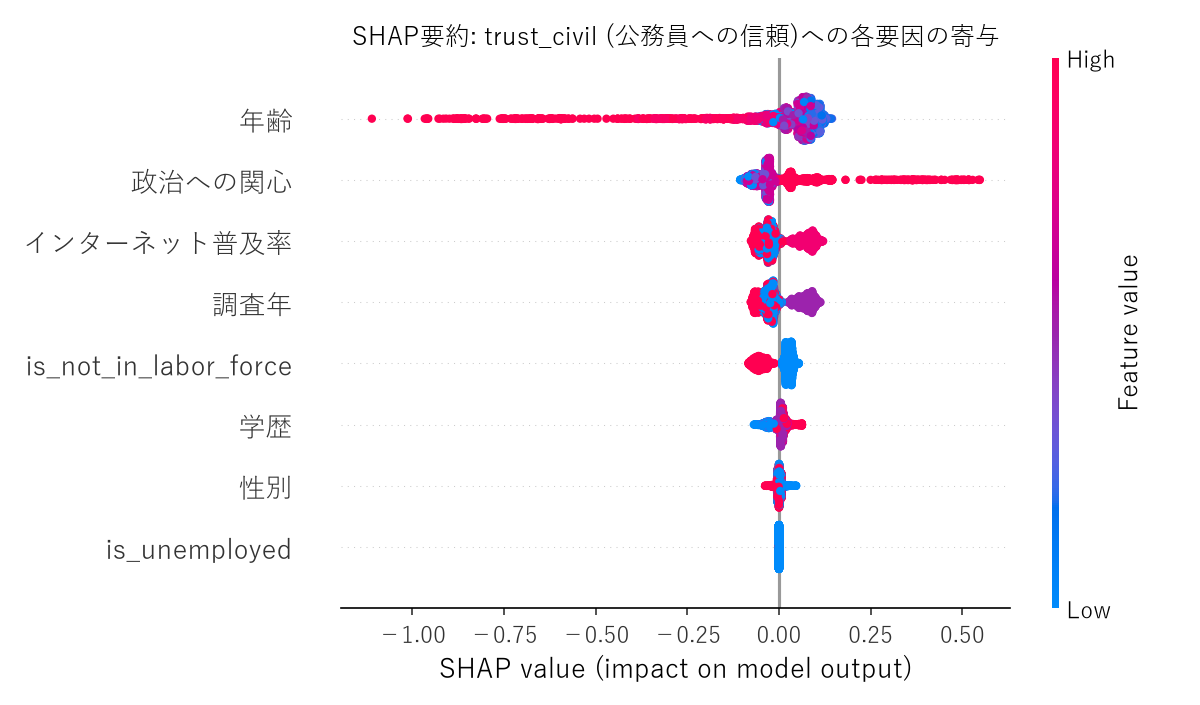
\includegraphics[width=0.85\textwidth]{shap_summary_trust_civil.png}
    \caption{SHAP要約プロット：公務員への信頼に対する各説明変数の寄与（Random Forest, ISSP）}
    \label{fig:shap-civil}
\end{figure}

\subsection{政治的態度クラスタの変化}
$K$-means（$K=3$，シルエット係数0.255で最適）により回答者を3クラスタに
分類したところ（corruption変数が存在する2006・2016年のみ，$N=2{,}340$），
「効力感・信頼・汚職認識・関心のいずれも低い」クラスタ0が2006年の25.8\%
から2016年の35.2\%へ約9.4ポイント増加した（図\ref{fig:cluster}）。

\begin{figure}[H]
    \centering
    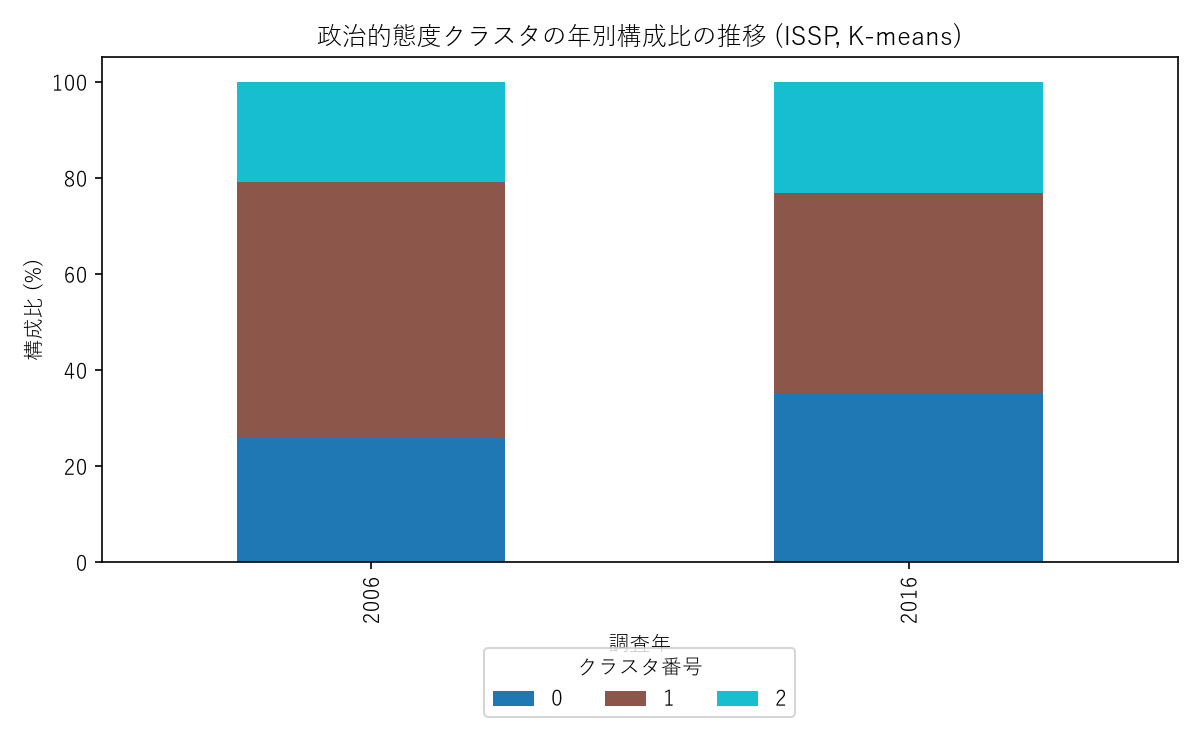
\includegraphics[width=0.7\textwidth]{cluster_profile.png}
    \caption{政治的態度クラスタの年別構成比（$K$-means, $K=3$）}
    \label{fig:cluster}
\end{figure}

\section{結果：WVS分析}

\subsection{制度への信頼の長期トレンド（1981--2019年）}
議会・公務員・政府・政党への信頼はいずれも，1980年代から2000年代半ばに
かけて緩やかに低下し，2005年前後に底を打ったのち上昇に転じ，2019年には
系列開始以来の最高水準に達している（図\ref{fig:wvs-trend}）。SNSが普及した
2010年代は，むしろ制度への信頼が長期的に\emph{回復}している時期にあたる。

\begin{figure}[H]
    \centering
    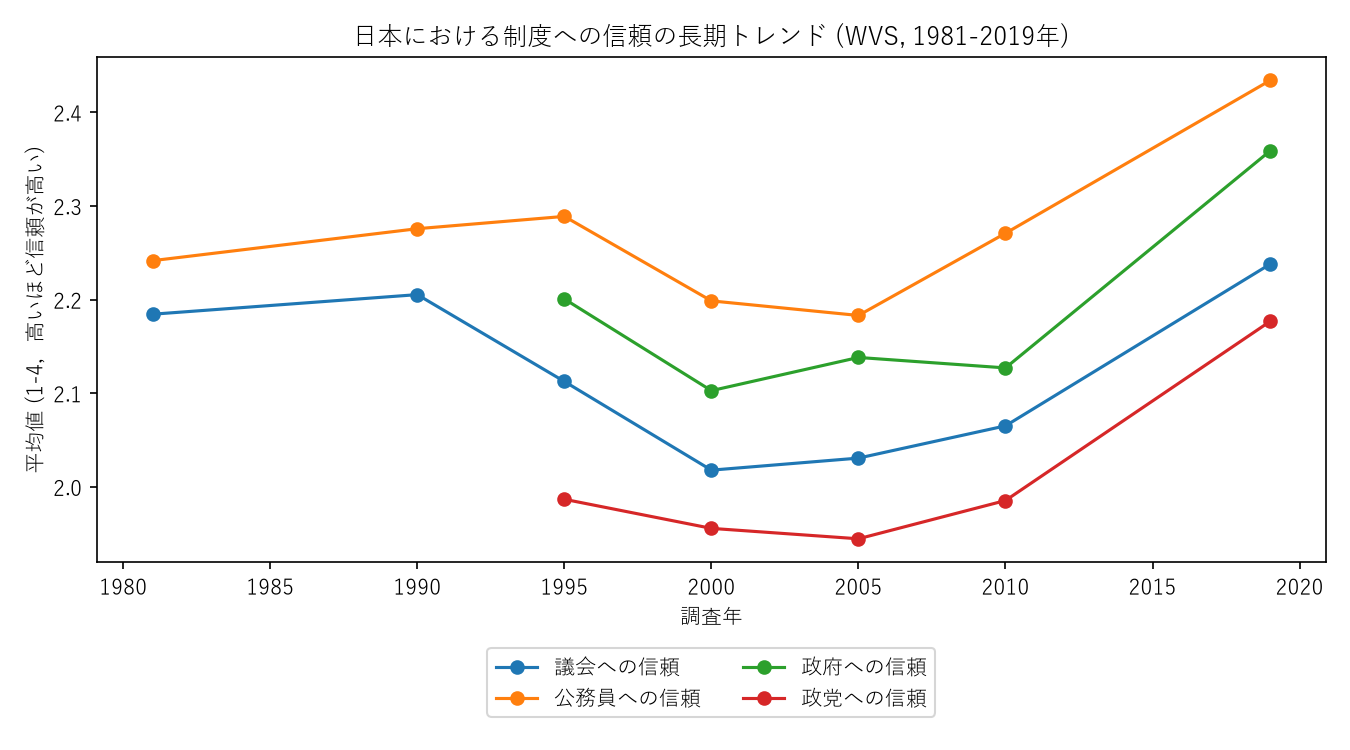
\includegraphics[width=0.85\textwidth]{wvs_trend.png}
    \caption{日本における制度への信頼の長期トレンド（WVS Time Series, 1981--2019年）}
    \label{fig:wvs-trend}
\end{figure}

\subsection{メディア利用（SNSを含む）が政治的信頼に与える影響}
Wave 6+7プール分析（インターネット・TV・新聞の3変数，SNS除く，
$N\approx2{,}700$）では，公務員信頼に対しインターネット利用（係数
$0.033$，$p<0.001$）と主観的所得水準（係数$0.072$，$p<0.001$）が有意な
正の効果を持った。これに対し，Wave 7限定分析（SNS利用を含む4変数，
$N\approx1{,}050$）では，\textbf{SNS利用頻度は議会信頼（$p=0.697$）・
公務員信頼（$p=0.915$）のいずれに対しても統計的に有意ではなかった}。
主観的所得水準は公務員信頼に対し係数$0.127$（$p<0.001$）と明確に有意
であった（表\ref{tab:wvs-wave7}）。SHAP分析（図\ref{fig:wvs-shap}）でも
SNS利用頻度の寄与は他の変数と比べて明確に小さい。

\begin{table}[H]
\centering
\caption{WVS Wave 7限定分析：OLS係数（$N\approx1{,}050$）}
\label{tab:wvs-wave7}
\begin{tabular}{lcccc}
\toprule
説明変数 & \multicolumn{2}{c}{議会信頼} & \multicolumn{2}{c}{公務員信頼} \\
 & 係数 & $p$ & 係数 & $p$ \\
\midrule
sns\_use            & $0.0055$  & 0.697 & $-0.0015$ & 0.915 \\
internet\_use       & $0.0012$  & 0.939 & $0.0132$  & 0.408 \\
tv\_news\_use       & $0.0728$  & 0.031* & $0.0287$ & 0.385 \\
newspaper\_use      & $0.0224$  & 0.134 & $0.0452$  & 0.002** \\
income\_level       & $0.0511$  & 0.100 & $0.1274$  & 0.000*** \\
is\_unemployed      & $-0.1660$ & 0.526 & $-0.2032$ & 0.428 \\
\bottomrule
\end{tabular}
\end{table}

\begin{figure}[H]
    \centering
    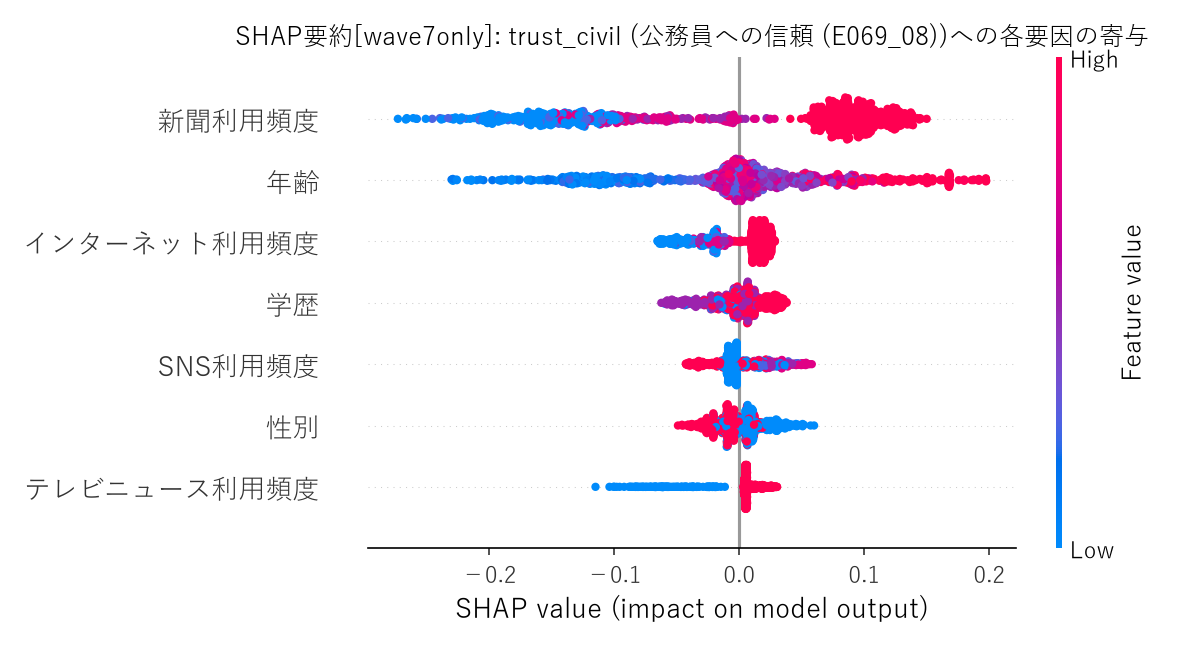
\includegraphics[width=0.85\textwidth]{wvs_shap_summary_trust_civil_wave7only.png}
    \caption{SHAP要約プロット：公務員への信頼に対する寄与（Random Forest, WVS Wave 7, SNS利用を含む）}
    \label{fig:wvs-shap}
\end{figure}

\textbf{この結果の含意}：経済的破壊への当事者性をより直接的に反映する
主観的所得水準を統制してもなお，SNS利用頻度の効果は非有意のままであった。
すなわちSNS利用の非有意性は「経済的要因を統制していないための見せかけの
結果」ではなく，所得という経済的要因を明示的にモデルへ含めても検出されない。

\subsection{5か国比較}
Wave 7限定分析の枠組みを米国・韓国・ドイツ・英国にも適用したところ
（表\ref{tab:cross-country}），SNS利用頻度が有意であったのは英国のみ
（議会信頼に対し係数$-0.0224$，$p=0.028$）。日・米・独ではいずれの
信頼指標に対しても非有意であり，SNS効果の非有意性は日本に固有の現象
ではないことが示された。

\begin{table}[H]
\centering
\caption{5か国比較：SNS利用頻度の議会・公務員信頼への効果（WVS Wave 7）}
\label{tab:cross-country}
\begin{tabular}{lcccc}
\toprule
 & \multicolumn{2}{c}{議会信頼} & \multicolumn{2}{c}{公務員信頼} \\
国 & SNS係数 & $p$ & SNS係数 & $p$ \\
\midrule
日本    & $+0.0044$ & 0.747 & $-0.0001$ & 0.997 \\
米国    & $+0.0049$ & 0.590 & $+0.0162$ & 0.102 \\
韓国    & $+0.0302$ & 0.070 & $+0.0155$ & 0.278 \\
ドイツ  & $+0.0066$ & 0.626 & $+0.0040$ & 0.735 \\
英国    & $-0.0224$ & 0.028* & $+0.0054$ & 0.621 \\
\bottomrule
\end{tabular}
\end{table}

\section{統計的限界}
以下の限界は，卒論本文の「統計的限界」の節で詳述している通りである。
(1) 内生性：メディア利用と政治的信頼の間には逆の因果関係が存在しうるが，
操作変数法等による識別は行っていない。(2) 除外変数：居住地・支持政党が
いずれのデータセットにも含まれていない。(3) WVS Wave 7限定分析は
$N\approx1{,}050$と相対的に小さく，単一時点の横断面データである。
(4) ISSPのインターネット普及率は実質的に調査年の代理に近く，同時期の
他の時間依存的要因からの識別が困難。(5) 多数の統計的検定を行っており，
多重比較の調整は行っていない。

\section{結論}
分析1全体を通じて，個人単位でSNS利用頻度を直接投入してもなお，制度への
信頼との間に統計的に有意な関連は見出せなかった。これは所得という経済的
要因を明示的に統制した場合や，日本以外の複数国で検証した場合にも頑健で
あった。この結果は「SNSは日本の政治に影響を与えていない」という強い
主張の根拠にはできないが，「制度への信頼という粗い態度指標だけでは，
SNS特有の動員メカニズムを十分に捉えられない」可能性を示唆しており，
より細かい言説レベルでの検証（分析2）へ進むための実証的な足がかりと
なる。

\end{document}
